\section{Camera mounts}
During the \preproject phase, I designed mounts for the \gls{gnss} antennas and sketched some camera mounts, as discussed and depicted in Sections 2.3.4 and 2.3.6 of the \preproject document.
However, during the manufacturing process of the camera mounts, it was observed that there was a slight amount of play or wiggle room, which can adversely affect the accuracy of stereo vision applications.

To address this issue, new camera mounts were designed and 3D printed.
The new mounts consist of two parts, and the distance between the interface with the cameras and the carbon fiber tubes was minimized to achieve a rigid connection.
Multiple iterations were developed, as shown in Figure \ref{fig:cam_mounts_iterations}, to achieve optimal tolerances and minimize any potential play or movement.


\begin{figure}[H]
    \centering
    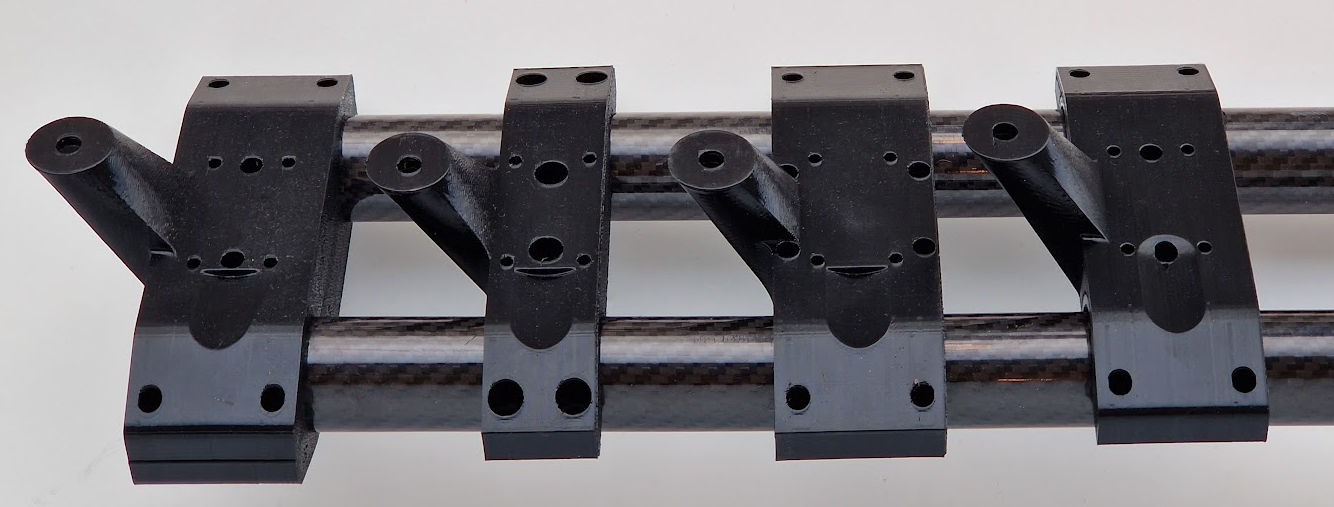
\includegraphics[width=\textwidth]{figures/3d_print/cam_mounts.png}
    \caption{Some iterations on the camera mount design}
    \label{fig:cam_mounts_iterations}
\end{figure}